\documentclass{standalone}
\usepackage{tikz}\usetikzlibrary{calc}
\begin{document}
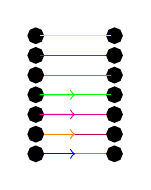
\begin{tikzpicture}[
  every node/.style={
    draw, circle, line width=3pt,
    outer sep=0pt, inner sep=1pt,
  },
]

  \def\drawNodes{
    \node (A) at (0,-\n*.25) {};
    \node (B) at (1,-\n*.25) {};
  }

  \def\n{0}\drawNodes
  \path [yellow] (A) edge (B);

  \def\n{1}\drawNodes
  \path [red] (A) edge [shorten >=1.5pt] (B);

  \def\n{2}\drawNodes
  \path [cyan] (A) edge [shorten <=1.5pt] (B);

  \def\n{3}\drawNodes
  \path [green] (A) edge [->] ($(A)!.5!(B)$) edge (B);

  \def\n{4}\drawNodes
  \path [magenta] (A) edge [->] ($(A)!.5!(B)$) edge [shorten >=1.5pt] (B);

  \def\n{5}\drawNodes
  \path (A) edge [->, shorten <=1.5pt, orange] ($(A)!.5!(B)$) ($(A)!.5!(B)$) edge [shorten >=1.5pt, purple] (B);

  \def\n{6}\drawNodes
  \path [brown, shorten <=1.5pt] (A) edge [shorten >=1.5pt] (B) edge [->, blue] ($(A)!.5!(B)$);
    
\end{tikzpicture}
\end{document}